\begin{name}
	{\tenchude}
	{\tendethi}
	{\tentruong}
	{\thoigian}
\end{name}
\setcounter{ex}{0}\setcounter{bt}{0}
\TN
\Opensolutionfile{ans}[ans/ansDe2-TN2]
\begin{ex}%[2-D1B1-SO-1-2425]%[VN-MT-7, Nguyễn Cao Cường]%[2D1N1-1]
	Cho hàm số $y=-x^3-3x^2+4$. Mệnh đề nào dưới đây đúng?
	\choice
	{Hàm số nghịch biến trên khoảng $(-2;0)$}
	{Hàm số đồng biến trên khoảng $(0;+\infty)$}
	{Hàm số đồng biến trên khoảng $(-\infty;-2)$}
	{\True Hàm số đồng biến trên khoảng $(-2;0)$}
	\loigiai{
		Tập xác định $\mathscr{D}=\mathbb{R}$.\\
		Ta có $y'=-3x^2-6x$.\\
		Xét $y'=0\Leftrightarrow -3x^2-6x=0\Leftrightarrow \hoac{&x=0\\&x=-2.}$\\
		Bảng biến thiên
		\begin{center}
			
\begin{tikzpicture}
				\tkzTabInit[nocadre=true,lgt=1,espcl=3,deltacl=0.5]
				{$x$/0.7,$y'$/0.7,$y$/2}
				{$-\infty$,$-2$,$0$,$+\infty$}
				\tkzTabLine{,-,0,+,0,-,}
				\tkzTabVar{+/$+\infty$,-/$0$,+/$4$,-/$-\infty$}
			\end{tikzpicture}
		\end{center}
		Hàm số đồng biến trên khoảng $(-2;0)$.
	}
\end{ex}

\begin{ex}%[2D1N1-2]
	Cho hàm số $f(x)$ có bảng biến thiên như sau
	\begin{center}
		
\begin{tikzpicture}
			\tkzTabInit[espcl=3,lgt=1,nocadre]
			{$x$/0.7,$y'$/0.7,$y$/2.1}
			{$-\infty$,$-1$,$0$,$1$,$+\infty$}
			\tkzTabLine{,+,0,-,0,+,0,-,}
			\tkzTabVar{-/$-\infty$,+/$2$,-/$-1$,+/$2$,-/$-\infty$}
		\end{tikzpicture}
	\end{center}
	Hàm số đã cho nghịch biến trên khoảng nào dưới đây?
	\choice
	{$(-\infty;1)$}
	{\True $(-1;0)$}
	{$(-\infty;0)$}
	{$(0;1)$}
	\loigiai{
		Từ bảng biến thên ta thấy trên khoảng $(-1;0)$ thì $f'(x) < 0$. \\
		Suy ra hàm số đã cho nghịch biến trên $(-1;0)$.
	}
\end{ex}

\begin{ex}%[CD12-KNTT, Mức độ 3]%[2D1V1-5]
	Một xe khách tuyến có sức chứa tối đa là $60$ hành khách. Nếu chuyến xe chở $x$ hành khách thì giá cho mỗi hành khách là $50\,000\left(3-\dfrac{x}{40}\right)^2$ (đồng). Doanh thu của xe tăng dần khi số hành khách $x$ nằm trong khoảng
	\choice
	{\True $(10;40)$}
	{$(20;50)$}
	{$(40;60)$}
	{$(0;60)$}
	\loigiai{
		Với $x\in [0;60]$, doanh thu của xe là \[f(x)=50\,000x\left(3-\dfrac{x}{40}\right)^2=50\,000x\left(9-\dfrac{3}{20}x+\dfrac{x^2}{1\,600}\right)=\dfrac{125x^3}{4}-7\,500x^2+450\,000x.\]
		Ta có $f'(x)=\dfrac{375x^2}{4}-15\,000x+45\,0000$, $f'(x)=0\Leftrightarrow \hoac{&x=120\notin [0;60]\\&x=40\in [0;60].}$\\
		Bảng biến thiên
		\begin{center}
			
\begin{tikzpicture}[scale=1, font=\footnotesize, line join=round, line cap=round, >=stealth]
				\tkzTabInit[nocadre=false, lgt=1.2, espcl=2, deltacl=0.8]
				{$x$/0.7, $f'(x)$/0.7,$f(x)$/2}
				{$0$, $40$, $60$}
				\tkzTabLine{,+,0,-,}
				\tkzTabVar{-/$0$,+/$8\,000\,000$,-/$6\,750\,000$}
			\end{tikzpicture}
		\end{center}
		Doanh thu của xe tăng dần khi số hành khách $x$ nằm trong khoảng $(10;40)$.
	}
\end{ex}
\begin{ex}%[2D1N2-1]
	Tìm điểm cực tiểu của đồ thị hàm số $ y=\dfrac{1}{3}{x^3}-2{x^2}+3x+1$.
	\choice
	{$x=1$}
	{\True $(3;1)$}
	{$x=3$}
	{$\left(1;\dfrac{7}{3}\right)$}
	\loigiai{
		Tập xác định: $\mathscr{D}=\mathbb{R}$.\\
		Ta có: $y'=x^2-4x+3=0\Leftrightarrow \hoac{&x=1\\&x=3.}$\\
		Lập bảng biến thiên:
		\begin{center}
			
\begin{tikzpicture}[scale=1, font=\footnotesize, line join=round, line cap=round, >=stealth]
				\tkzTabInit[nocadre,lgt=1.2,espcl=2.5,deltacl=0.6]
				{$x$/0.6,$f'(x)$/0.6,$f(x)$/2.5}
				{$-\infty$,$1$,$3$,$+\infty$}
				\tkzTabLine{,+,0,-,0,+,}
				\tkzTabVar{-/$-\infty$,+/$\dfrac{7}{3}$,-/$1$,+/$+\infty$}
			\end{tikzpicture}
		\end{center}
		Dựa vào BBT suy ra, điểm cực tiểu của đồ thị hàm số là $(3;1)$.
	}
\end{ex}

\begin{ex}%[2D1N2-2]
	\immini{
	Cho hàm số $y=f(x)$ có đồ thị như hình bên. \\Phát biểu nào sau đây là đúng?
	\choice
	{$y_{\text{CT}}=1,y_{\text{CĐ}}=2$}
	{$y_{\text{CT}}=2,y_{\text{CĐ}}=-1$}
	{$y_{\text{CT}}=-2,y_{\text{CĐ}}=2$}
	{\True $y_{\text{CT}}=2,y_{\text{CĐ}}=-2$}
	}{
	\begin{tikzpicture}[scale=0.5,>=stealth, font=\footnotesize, line join=round, line cap=round]
		\draw[->] (-6,0)--(6,0)node[below]{$x$};
		\draw[->] (0,-6)--(0,6)node[left]{$y$};
		\draw[samples=100,domain=-5:-0.18] plot (\x,{(\x)+1/(\x)});
		\draw[samples=100,domain=0.2:5] plot (\x,{(\x)+1/(\x)});
		\draw[samples=100,domain=-5:5] plot (\x,{(\x)});
		\draw(0,0)node[below right]{$O$};
		\draw[dashed]
		(-1,0)node[below left]{$-1$}
		(0,-2)node[right]{$-2$}
		(0,2)node[above left]{$2$}
		(1,0)node[below right]{$1$}
		(1,0)--(1,2)--(0,2)
		(-1,0)--(-1,-2)--(0,-2)
		;
	\end{tikzpicture}
	}
	\loigiai{
		Dựa vào đồ thị ta thấy hàm số có $y_{\text{CT}}=2, y_{\text{CĐ}}=-2$.
	}
\end{ex}

\begin{ex}%[2D1H2-1]
	Biết đồ thị hàm số $y=x^3-3x+1$ có hai điểm cực trị $A$, $B$. Khi đó phương trình đường thẳng $AB$ là
	\choice
	{$y=x-2$}
	{$y=2x-1$}
	{\True $y=-2x+1$}
	{$y=-x+2$}
	\loigiai{
		Phương pháp tự luận:\\
		Phương trình $y'=0\Leftrightarrow 3x^2-3=0\Leftrightarrow\hoac{&x=-1\\&x=1.}$\\
		Suy ra $A(1;-1)$, $B(-1;3)$ nên phương trình của đường thẳng $AB$ là $y=-2x+1$.\\
		Phương pháp trắc nghiệm:\\
		Cách $1$:\\
		Lấy $\dfrac{y}{y'}=\dfrac{x^3-3x+1}{3x^2-3} =\left(\dfrac{1}{3}x\right)\cdot\left(3x^2-3\right)-2x+1$\\
		Phương trình của đường thẳng $AB$ là $y=-2x+1$.\\
		Cách $2$:\\
		Lấy $y-\dfrac{y'\cdot y''}{18a}=x^3-3x+1-\dfrac{\left(3x^2-3\right)\cdot 6x}{18}=-2x+1$.\\
		Phương trình của đường thẳng $AB$ là $y=-2x+1$.\\
		Cách $3$: Bấm máy tính:\\
		Bước $1$: Bấm Mode $2$ (CMPLX)\\
		Bước $2$:	Nhập $x^3-3x+1-\left(3x^2-3\right)\dfrac{x}{3}$ \\
		Bước $3$: CALC $x=i$\\
		Kết quả: $1-2i$ suy ra phương trình $AB\colon y=-2x+1$.}
\end{ex}

\begin{ex}%[2D1H3-1]
	Giá trị lớn nhất của hàm số $y=\dfrac{x^2-3x+3}{x-1}$ trên đoạn $\left[-2;\dfrac{1}{2}\right]$ là
	\choice
	{$-\dfrac{7}{2}$}
	{$-\dfrac{13}{3}$}
	{$1$}
	{\True $-3$}
	\loigiai{
		Ta có $y=f(x)=\dfrac{x^2-3x+3}{x-1}$ liên tục trên $\left[-2;\dfrac{1}{2}\right]$.\\
		Đạo hàm $y'=\dfrac{(2x-3)(x-1)-(x^2-3x+3)}{(x-1)^2}=\dfrac{x^2-2x}{(x-1)^2}$, xác định với mọi $x\neq 1$.\\
		$y'=0\Leftrightarrow \hoac{&x=0\in\left[-2;\dfrac{1}{2}\right]\\&x=2\not\in\left[-2;\dfrac{1}{2}\right]}$.\\
		Ta có $f(-2)=-\dfrac{13}{3}, f(0)=-3, f\left(\dfrac{1}{2}\right)=-\dfrac{7}{2}$.\\
		Vậy $\max\limits_{\left[-2;\frac{1}{2}\right]}y=-3$ tại $x=0$.
	}
\end{ex}

\begin{ex}%[2D1N4-1]
	Cho hàm số $y=f(x)$ có đồ thị là đường cong $(C)$ và các giới hạn $\lim\limits_{x\to 2^{+}}f(x)=1$, $\lim\limits_{x\to 2^{-}}f(x)=1$, $\lim\limits_{x\to +\infty}f(x)=2$, $\lim\limits_{x\to -\infty}f(x)=2$. Hỏi mệnh đề nào sau đây đúng?
	\choice
	{\True Đường thẳng $y=2$ là tiệm cận ngang của $(C)$}
	{Đường thẳng $y=1$ là tiệm cận ngang của $(C)$}
	{Đường thẳng $x=2$ là tiệm cận ngang của $(C)$}
	{Đường thẳng $x=2$ là tiệm cận đứng của $(C)$}
	\loigiai{
		Ta có $\lim\limits_{x\to +\infty}f(x)=2$, $\lim\limits_{x\to -\infty}f(x)=2\Rightarrow y=2$ là tiệm cận ngang của $(C)$.
	}
\end{ex}

\begin{ex}%[Dự án TL12New-4in1-NCT]%[2D1H4-1]
	\immini{Cho hàm số $f(x)$ có đồ thị như hình vẽ bên. Tiệm cận đứng và tiệm cận ngang của đồ thị hàm số lần lượt là
		\choice
		{$x=1$ và $y=-2$}
		{\True $x=-1$ và $y=2$}
		{$x=1$ và $y=2$}
		{$x=-1$ và $y=-2$}}
	{
		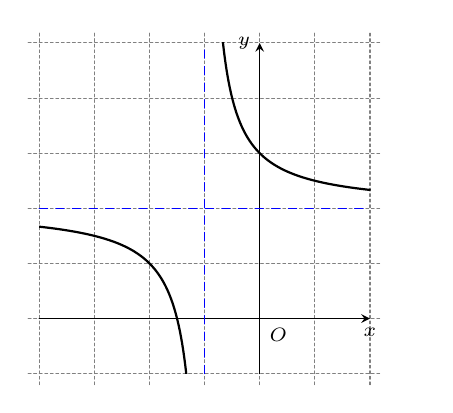
\begin{tikzpicture}[>=stealth,line join=round,line cap=round, font=\footnotesize,scale=0.7]
			\def\a{2}
			\def\b{3}
			\def\c{1}
			\def\d{1}
			\draw[color=gray,dash pattern=on 1pt off 1pt,xstep=1.0cm,ystep=1.0cm] (-4.2,-1.2) grid (2.2,5.2);
			\draw[->] (-4,0) -- (2,0) node[below] {\scriptsize $x$};
			\draw[->] (0,-1) -- (0,5) node[left] {\scriptsize $y$};
			\draw (0,0)node[below right]{\scriptsize $O$};
			\draw[dashed,blue] (-1,-1)--(-1,5) (-4,2)--(2,2); % Vẽ tiệm cận đứng và TCN
			\clip (-4,-1)rectangle(3,5);
			\pgfmathsetmacro{\can}{-(\d)/(\c)}
			\draw[thick,samples=150,smooth,domain=-4:{\can-.1}] plot(\x,{(\a*\x+(\b))/(\c*\x+(\d))}); % Vẽ nhánh bên trái tiệm cận đứng
			\draw[thick,samples=150,smooth,domain={\can+.1}:2] plot(\x,{(\a*\x+(\b))/(\c*\x+(\d))}); % Vẽ nhánh bên phải tiệm cận đứng
		\end{tikzpicture}
	}
	\loigiai{
		Nhìn vào đồ thị ta suy ra ngay tiệm cận đứng và tiệm cận ngang lần lượt là các đường thẳng $x=-1$; $y=2$.}
\end{ex}

\begin{ex}%[2D1V4-1]
	Tổng số đường tiệm cận đứng và tiệm cận ngang của đồ thị hàm số $y=\dfrac{\sqrt{2-x}+x}{x^2-4}$ là
	\choice
	{\True $2$}
	{$1$}
	{$0$}
	{$3$}
	\loigiai{
		Tập xác định của hàm số là $\mathscr{D}=(-\infty;2)\setminus \{-2\}$.\\
		Ta có
		\begin{itemize}
			\item $\lim\limits_{x\to -\infty}y=\lim\limits_{x\to -\infty}\dfrac{\sqrt{\dfrac{2}{x^3}-\dfrac{1}{x^3}}+\dfrac{1}{x}}{1-\dfrac{4}{x^2}}=0\Rightarrow y=0$ là đường tiệm cận ngang.
			\item $\lim\limits_{x\to 2^-}y=\lim\limits_{x\to 2^-}\dfrac{\sqrt{2-x}+x}{x^2-4}=-\infty\Rightarrow x=2$ là đường tiệm cận đứng.
			\item $\lim\limits_{x\to (-2)^-}y=\lim\limits_{x\to (-2)^-}\dfrac{2-x-x^2}{(x+2)(x-2)(\sqrt{2-x}-x)}=\lim\limits_{x\to (-2)^-}\dfrac{(1-x)}{(x-2)(\sqrt{2-x}-x)}=-\dfrac{3}{16}$.
			\item $\lim\limits_{x\to (-2)^+}y=\lim\limits_{x\to (-2)^+}\dfrac{2-x-x^2}{(x+2)(x-2)(\sqrt{2-x}-x)}=\lim\limits_{x\to (-2)^+}\dfrac{(1-x)}{(x-2)(\sqrt{2-x}-x)}=-\dfrac{3}{16}$.\\
			      Suy ra $x=-2$ không phải là đường tiệm cận đứng.
		\end{itemize}
		Vậy tổng số đường tiệm cận đứng và tiệm cận ngang của đồ thị hàm số là $2$.
	}
\end{ex}

\begin{ex}%[Dự án Giảng 12 Nhóm Toán & LaTex, Lê Minh Thiện Anh]%[2D1N5-1]
	\immini{Đường cong bên là đồ thị của một trong bốn hàm số đã cho sau đây. Hỏi đó là hàm số nào?
		\choice
		{$y=-x^3+x^2-2$}
		{\True $y=x^3+3x^2-2$}
		{$y=x^3-3x+2$}
		{$y=x^2-3x-2$}
	}{
		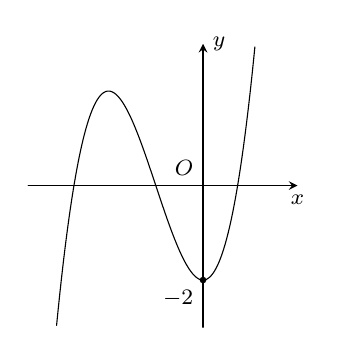
\begin{tikzpicture}[scale=0.6, font=\footnotesize,line join=round, line cap=round,>=stealth]
			\draw[->] (-3.7,0.) -- (2,0) node[below]{$x$};
			\draw[->] (0,-3) -- (0,3) node[right]{$y$};
			\fill (0,0) node[above left]{$O$};
			\fill (0,-2) circle(2pt) node[below left]{$-2$};
			\draw[smooth,samples=300,domain=-3.1:1.1] plot(\x,{(\x+2)^3-3*(\x+2)^2+2});
		\end{tikzpicture}
	}
	\loigiai{
		Dựa vào hình dáng đồ thị, ta thấy đây là đồ thị của hàm số bậc ba $y=ax^3+bx^2+cx+d$ với $a>0$ nên loại các hàm $y=x^2-3x-2$, $y=-x^3+x^2-2$.\\
		Mặt khác, đồ thị đi qua điểm $(0;-2)$ nên loại hàm $y=x^3-3x+2$.
	}
\end{ex}

\begin{ex}%[2D1N5-7]%[DA- EX-TF-TLN2024 - Phạm Quốc Toàn]
	Điểm nào sau đây thuộc đồ thị hàm số $\left(C \right) \colon y=\dfrac{x^2+3x+3}{x+1}$?
	\choice
	{$\left(3;0 \right)$}
	{$\left(-2;1 \right)$}
	{\True $\left(0;3 \right)$}
	{$\left(2;1 \right)$}
	\loigiai{
		Với $x=0$, ta có $y=3$. Vậy điểm $\left(0;3 \right)$ thuộc đồ thị $\left(C \right)$.
	}
\end{ex}

\begin{ex}%[2D1H5-1]%[DỰ ÁN NGÂN HÀNG HỎI 2024 - K12 - HỒ VĂN TRUNG]
	Đường cong trong hình dưới đây là đồ thị của hàm số nào
	\begin{center}
		\begin{tikzpicture}
			\draw[->] (-1.5,0)--(3,0) node [below]{$x$};
			\draw[->] (0,-2)--(0,3.5) node [left]{$y$};
			\path[] (0,0) node [above left=1pt]{$O$};
			\clip (-1.5,-2) rectangle (3,3.5);
			\draw[smooth, samples=100] plot (\x, {(\x)^3-3*(\x)^2+3});
		\end{tikzpicture}
	\end{center}
	\choice
	{\True $y=x^3-3x^2+3$}
	{$y=-x^3+3x^2+3$}
	{$y=x^4-2x^2+3$}
	{$y=-x^4+2x^2+3$}
	\loigiai{
		Đồ thị đã cho là hàm số bậc $3$, có hệ số $a>0$.
	}
\end{ex}

\begin{ex}%[2D1V5-8]
	Sau khi phát hiện một bệnh dịch, các chuyên gia y tế ước tính số người nhiễm bệnh tại thời điểm xuất hiện bệnh nhân đầu tiên đến ngày thứ $t$ là $f(t)=4 t^{3}-\dfrac{t^{4}}{2}$ (người).  Nếu xem $f'(t)$ là tốc độ truyền bệnh (người/ngày) tại thời điểm $t$ với $t \in[0 ; 6]$. Tốc độ truyền bệnh sẽ lớn nhất vào ngày thứ mấy?
	\choice
	{$5$}
	{$3$}
	{$6$}
	{\True $4$}
	\loigiai{
	Ta có $g(t)=f'(t)=12 t^{2}-2 t^{3}$ với $t \in[0 ; 6]$. \\
	$g'(t)=24 t-6 t^{2}$; $g'(t)=0 \Leftrightarrow  24  t-6 t^{2}=0 \Leftrightarrow\hoac{&t=0 \\&t=4.}$ \\
	Khi đó{,} $g(0)=0 ; g(4)=64 ; g(6)=0$. \\
	Vậy tốc độ truyền bệnh sẽ lớn nhất vào ngày thứ $4$.
	}
\end{ex}

\begin{ex}%[2D1H3-6]%[Tổ 17 - Đợt 16 - Chương 1 - Ôn tập chương - KNTT - Đề 3]%[Nguyễn Nhan Gia Hưng]
	Một chất điểm chuyển động thẳng với phương trình $s(t)=t^3+3t-1$, trong đó $t$ tính bằng giây và $s(t)$ tính bằng mét. Tính vận tốc của chất điểm tại thời điểm $t=5$ (giây)?
	\choice
	{$139$ (m/s)}
	{\True $78$ (m/s)}
	{$30$ (m/s)}
	{$77$ (m/s)}
	\loigiai{Ta có $v(t)=s^{\prime}(t)=3 t^{2}+3$.\\
	Vận tốc của chất điểm tại thời điểm $t=5$ là $v(5)=3\cdot 5^2+3=78$ (m/s).
	}
\end{ex}

\begin{ex}%[2D1H3-6]%[Dự án 2025-K12-TL-TY]%[Thành Đức Trung]
	Một vật chuyển động theo quy luật $s=-\dfrac{1}{2}t^3+6t^2$ với $t$ (giây) là khoảng thời gian tính từ khi vật bắt đầu chuyển động và $s$ (mét) là quãng đường vật di chuyển được trong khoảng thời gian đó. Hỏi trong khoảng thời gian $6$ giây, kể từ khi bắt đầu chuyển động, vận tốc lớn nhất của vật đạt được bằng bao nhiêu?
	\choice
	{\True $24$ m/s}
	{$108$ m/s}
	{$18$ m/s}
	{$64$ m/s}
	\loigiai
	{
		Ta có $v(t) = S'(t) = -\dfrac{3}{2}t^2 +12t$ m/s.\\
		Vì xét trong khoảng thời gian $6$ giây, kể từ lúc bắt đầu chuyển động nên ta có $0<t\leq 6$.\\
		Ta có $v'(t) = -3t +12$. \\
		Xét $v'(t) = 0 \Leftrightarrow t = 4$.\\
		Bảng biến thiên
		\begin{center}
			
\begin{tikzpicture}
				\tkzTabInit[nocadre=false,lgt=1.2,espcl=2.5,deltacl=0.6]
				{$t$ /0.6,$v'$ /0.6,$v$ /2}
				{$0$,$4$,$6$}
				\tkzTabLine{,+,0,-,}
				\tkzTabVar{-/$0$, +/$24$,-/$18$}
			\end{tikzpicture}
		\end{center}
		Vậy vật đạt vận tốc lớn nhất bằng $24$ m/s khi $t=4$ s.
	}
\end{ex}

\begin{ex}%[2H2N1-1]
	Trong không gian $Oxyz$, cho điểm $A (3;1; 2)$. Điểm đối xứng của $A$ qua $O$ có tọa độ là
	\choice
	{$(3;2;1) $}
	{$(-2;-1;-3) $}
	{\True $(-3;-1;-2) $}
	{$(2;1;3) $}
	\loigiai{Gọi $A'$ là điểm đối xứng của $A$ qua $O$, khi đó $O$ là trung điểm của $AA'$.\\
		Vậy $A'(-3;-1;-2) .$
	}
\end{ex}

\begin{ex}%[Trần Quang Trường-Hình học 12-Chương 2]%[2H2N1-2]
	Trên đoạn thẳng $A B$, lấy điểm $M$ sao cho $A B=3 A M$ như hình vẽ sau:
	\begin{center}
		\begin{tikzpicture}[>=stealth,line join=round,line cap=round,font=\footnotesize,scale=1]
			\coordinate[label=below left:$A$](A) at (0,0);
			\coordinate[label=below right:$B$](B) at (6,0);
			\coordinate[label = below:$M$] (M) at ($(A)!1/3!(B)$);
			\draw (A)--(B);
			\fill[black] (A) circle (1.5pt) (B) circle (1.5pt) (M) circle (1.5pt);
		\end{tikzpicture}
	\end{center}
	Mệnh đề nào sau đây đúng?
	\choice
	{$\overrightarrow{M B}=2 \overrightarrow{M A}$}
	{$\overrightarrow{M A}=2 \overrightarrow{M B}$}
	{\True $\overrightarrow{M B}=-2 \overrightarrow{M A}$}
	{$\overrightarrow{M A}=-2 \overrightarrow{M B}$}
	\loigiai{
		Dựa vào giả thiết và hình vẽ ta có $\overrightarrow{M B}=-2 \overrightarrow{M A}$.
	}
\end{ex}

\begin{ex}%[2-H2B4-SO-13-2425 (Nguồn Đề 13 - )]%[VN-MT-7, Lê Văn Hiếu]%[2H2N1-3]
	Cho tứ diện đều $ABCD$ có cạnh bằng $2$. Tính $\overrightarrow{AB}\cdot\overrightarrow{CD}$.
	\choice
	{$\overrightarrow{AB}\cdot\overrightarrow{CD}=-4$}
	{$\overrightarrow{AB}\cdot\overrightarrow{CD}=2$}
	{$\overrightarrow{AB}\cdot\overrightarrow{CD}=1$}
	{\True $\overrightarrow{AB}\cdot\overrightarrow{CD}=0$}
	\loigiai{
		Vì $ABCD$ là tứ diện đều nên các tam giác $ABC$ và $ABD$ là các tam giác đều.\\
		Khi đó
		\begin{eqnarray*}
			\overrightarrow{AB}\cdot\overrightarrow{CD}&=&\overrightarrow{AB}\cdot(\overrightarrow{AD}-\overrightarrow{AC})\\
			&=&\overrightarrow{AB}\cdot\overrightarrow{AD}-\overrightarrow{AB}\cdot\overrightarrow{AC}\\
			&=&2\cdot2\cdot\cos60^\circ-2\cdot2\cdot\cos60^\circ=0.
		\end{eqnarray*}
	}\end{ex}

\begin{ex}%[2H2H1-2]
	Cho hình tứ diện $ABCD$ có trọng tâm $G$. Mệnh đề nào sau đây \textbf{sai}.
	\choice
	{\True $\overrightarrow{AG}=\dfrac{2}{3}\left( \overrightarrow{AB}+\overrightarrow{AC}+\overrightarrow{AD} \right)$}
	{ $\overrightarrow{AG}=\dfrac{1}{4}\left( \overrightarrow{AB}+\overrightarrow{AC}+\overrightarrow{AD} \right)$}
	{ $\overrightarrow{OG}=\dfrac{1}{4}\left( \overrightarrow{OA}+\overrightarrow{OB}+\overrightarrow{OC}+\overrightarrow{OD} \right)$}
	{ $\overrightarrow{GA}+\overrightarrow{GB}+\overrightarrow{GC}+\overrightarrow{GD}=\overrightarrow{0}$}
	\loigiai{
		Theo giả thuyết trên thì với $O$ là một điểm bất kỳ ta luôn có \[\overrightarrow{OG}=\dfrac{1}{4}\left( \overrightarrow{OA}+\overrightarrow{OB}+\overrightarrow{OC}+\overrightarrow{OD} \right).\]
		Ta thay điểm $O$ bởi điểm $A$ thì ta có
		\[\overrightarrow{AG}=\dfrac{1}{4}\left( \overrightarrow{AA}+\overrightarrow{AB}+\overrightarrow{AC}+\overrightarrow{AD} \right)\Leftrightarrow \overrightarrow{AG}=\dfrac{1}{4}\left( \overrightarrow{AB}+\overrightarrow{AC}+\overrightarrow{AD} \right).\]
		Do vậy $\overrightarrow{AG}=\dfrac{2}{3}\left( \overrightarrow{AB}+\overrightarrow{AC}+\overrightarrow{AD} \right)$ là sai.}
\end{ex}

\begin{ex}%[2-H2B1-SO-1-2425]%[VN-MT-7, Huỳnh Thanh Chí]%[2H2H1-3]
	Cho hình hộp $ABCD.A'B'C'D'$. Đẳng thức sau đây là {\bf sai}?
	\choice
	{$\overrightarrow{AC'}=\overrightarrow{AB}+\overrightarrow{AD}+\overrightarrow{AA'}$}
	{$\overrightarrow{AB}=\overrightarrow{D'C'}$}
	{\True $\overrightarrow{AB}+\overrightarrow{AA'}=\overrightarrow{AD}+\overrightarrow{DD'}$}
	{$\overrightarrow{AD}+\overrightarrow{DC}+\overrightarrow{CC'}=\overrightarrow{AD'}+\overrightarrow{D'C'}$}
	\loigiai{
		\begin{center}
			\begin{tikzpicture}[scale=0.9,font=\footnotesize,line join=round,line cap=round,>=stealth]
				\def\a{3.5}
				\def\h{4}
				\path (0:0) coordinate (A)
				++(0:\a) coordinate (D)
				++(-130:\a/2) coordinate (C)
				($(A)+(C)-(D)$) coordinate (B)
				($(A)!0.25!(C)$) coordinate (H)
				($(H)+(90:\h)$) coordinate (A')
				($(A')+(C)-(A)$) coordinate (C')
				($(C')+(B)-(C)$) coordinate (B')
				($(A')+(D)-(A)$) coordinate (D')
				($(A)!0.5!(C)$) coordinate (O)
				;
				\draw[dashed] (B)--(A)--(D) (A)--(A');
				\draw (C)--(C') (D)--(D') (B)--(B') (B)--(C)--(D) (A')--(B')--(C')--(D')--cycle;
				\foreach \x/\g in {A/180,B/180,C/0,D/0,A'/180,B'/180,C'/0,D'/0}
				\fill (\x) circle (1pt)
				($(\g:4mm)+(\x)$) node {$\x$};
				% \draw pic[draw,angle radius=2mm]{right angle=A'--H--C};%Theo chiều dương
			\end{tikzpicture}
		\end{center}
		Xét đẳng thức $\overrightarrow{AB}+\overrightarrow{AA'}=\overrightarrow{AD}+\overrightarrow{DD'}$ mà $\overrightarrow{AA'}=\overrightarrow{DD'}$ suy ra $\overrightarrow{AB}=\overrightarrow{AD}$ (sai).\\
		Do đó, đẳng thức $\overrightarrow{AB}+\overrightarrow{AA'}=\overrightarrow{AD}+\overrightarrow{DD'}$ sai.
	}
\end{ex}

\begin{ex}%[2H2H1-1]
	Cho ba vectơ $\vec{a}, \vec{b}, \vec{c}$. Trong các mệnh đề sau, mệnh đề nào sai?
	\choice
	{Nếu $\vec{a}, \vec{b}, \vec{c}$ không đồng phẳng thì từ $m \vec{a}+n \vec{b}+p \vec{c}=\overrightarrow0$ ta suy ra $m=n=p=0$}
	{Nếu có $m \vec{a}+n \vec{b}+p \vec{c}=\overrightarrow0$, trong đó $m^2+n^2+p^2> 0$ thì $\vec{a}, \vec{b}, \vec{c}$ đồng phẳng}
	{Với ba số thực $m, n, p$ thỏa mãn $m+n+p \neq 0$ ta có $m \vec{a}+n \vec{b}+p \vec{c}=\overrightarrow0$ thì $\vec{a}, \vec{b}, \vec{c}$ đồng phẳng}
	{\True Nếu giá của $\vec{a}, \vec{b}, \vec{c}$ đồng qui thì $\vec{a}, \vec{b}, \vec{c}$ đồng phẳng}
	\loigiai{
		Nếu giá của $\vec{a}, \vec{b}, \vec{c}$ đồng qui thì $\vec{a}, \vec{b}, \vec{c}$ đồng phẳng là sai. Ví dụ phản chứng $3$ cạnh của hình chóp tam giác đồng qui tại $1$ đỉnh nhưng chúng không đồng phẳng.
	}
\end{ex}

\begin{ex}%[2H2V1-3] 2
	Trong các khẳng định sau, khẳng định nào \textbf{sai}?
	\choice
	{\True Nếu giá của ba vectơ $\overrightarrow{a},\overrightarrow{b},\overrightarrow{c}$ cắt nhau từng đôi một thì ba vectơ đó đồng phẳng}
	{Nếu trong ba vectơ $\overrightarrow{a},\overrightarrow{b},\overrightarrow{c}$ có một vectơ $\overrightarrow{0}$ thì ba vectơ đó đồng phẳng}
	{Nếu giá của ba vectơ $\overrightarrow{a},\overrightarrow{b},\overrightarrow{c}$ cùng song song với một mặt phẳng thì ba vectơ đó đồng phẳng}
	{Nếu trong ba vectơ $\overrightarrow{a},\overrightarrow{b},\overrightarrow{c}$ có hai vectơ cùng phương thì ba vectơ đó đồng phẳng.
	}
	\loigiai{
		+ Nắm vững khái niệm ba véctơ đồng phẳng} \end{ex}

\begin{ex}%[2H2N2-2]NEWID%[Tổ 17 - Đợt 17 - Chương 2 - - CTST - Đề 2]%[Trần Chánh Nghĩa]
	Cho tam giác $ABC$, biết $A (1;-2;4 )$, $B (0;2;5 )$, $C (5;6;3 )$. Tọa độ trọng tâm $G$ của tam giác $ABC$ là
	\choice
	{\True $G (2;2;4 )$}
	{$G (4;2;2 )$}
	{$G (3;3;6 )$}
	{$G (6;3;3 )$}
	\loigiai
	{
	$G$ là trọng tâm của tam giác $ABC$ nên ta có:
	$\heva{
		{{x}_{G}}= \dfrac{1+0+5}{3}=2  \\
		{{y}_{G}}= \dfrac{-2+2+6}{3}=2  \\
		{{z}_{G}}= \dfrac{4+5+3}{3}=4  \\
		}$.\\
	Vậy $G (2;2;4 )$.
	}
\end{ex}

\begin{ex}%[Mui Doan, dự án 12EX-OTTN2025]%[2H2N2-1]
	Trong không gian $Oxyz$, khoảng cách giữa hai điểm $A(x_1; y_1; z_1)$ và $B(x_2; y_2; z_2)$ bằng
	\choice
	{$|x_2-x_1|+|y_2-y_1|+|z_2-z_1|$}
	{\True  $\sqrt{(x_2-x_1)^2+(y_2-y_2)^2+(z_2-z_1)^2}$}
	{$\dfrac{|x_2-x_1|+|y_2-y_1|+|z_2-z_1|}{3}$}
	{$\sqrt{\dfrac{(x_2-x_1)^2+(y_2-y_2)^2+(z_2-z_1)^2}{3}}$}
	\loigiai{
		Công thức tính khoảng cách giữa hai điểm là $AB=\sqrt{(x_2-x_1)^2+(y_2-y_2)^2+(z_2-z_1)^2}$.
	}
\end{ex}

\begin{ex}%[2-H2B3-SO-9-2425]%[VN-MT-7, Nguyễn Trường Vinh]%[2H2N2-4]
	Trong không gian với hệ trục tọa độ $Oxyz$, tích vô hướng của hai vectơ $\overrightarrow{m}=(a;b;c)$ và $\overrightarrow{n}=(x;y;z)$ được xác định bởi công thức nào sau đây?.
	\choice
	{\True $\overrightarrow{m}\cdot \overrightarrow{n}=ax+by+cz$}
	{$\overrightarrow{m}\cdot \overrightarrow{n}=ax-by+cz$}
	{$\overrightarrow{m}\cdot \overrightarrow{n}=\sqrt{a^2+b^2+c^2}\cdot \sqrt{x^2+y^2+z^2}$}
	{$\overrightarrow{m}\cdot \overrightarrow{n}={{(x-a)}^2}+{{(y-b)}^2}+{{(z-c)}^2}$}
	\loigiai{
		Ta có $\overrightarrow{m}\cdot \overrightarrow{n}=ax+by+cz$.}
\end{ex}

\begin{ex}%[2H2H2-1]
	Trong không gian với hệ tọa độ $Oxyz$, cho $3$ vectơ $\vec{a}=\left(2;-5;3\right)$, $\vec{b}=\left(0;2;-1\right)$, $\vec{c}=\left(1;7;2\right)$. Tìm tọa độ $\vec{d}=\vec{a}-4\vec{b}-2\vec{c}$.
	\choice
	{\True $\left(0;-27;3\right)$}
	{$\left(1;2;-7\right)$}
	{$\left(0;27;3\right)$}
	{$\left(0;27;-3\right)$}
	\loigiai{
		Ta có $\vec{a}=\left(2;-5;3\right),4\vec{b}=\left(0;8;-4\right),2\vec{c}=\left(2;14;4\right)$.\\
		Suy ra $\vec{d}=\left(2-0-2;-5-8-14;3-(-4)-4\right)=\left(0;-27;3\right)$.
	}
\end{ex}

\begin{ex}%[BG12 New, Anh Duy]%[2H2H2-4]
	Trong không gian $Oxyz$, cho $A(-1;2;4)$, $B(-1;1;4)$, $C(0;0;4)$. Tìm số đo $\widehat{ABC}$.
	\choice
	{$45^\circ $}
	{$60^\circ $}
	{\True $135^\circ $}
	{$120^\circ $}
	\loigiai{
		Ta có $\vec{BA}=(0;1;0)$, $\vec{BC}=(1;-1;0)$ nên $\vec{BA}\cdot \vec{BC}=-1$.\\
		Lại có $\left| \vec{BA}\right|=\sqrt{0^2+1^2+0^2}=1$ và $\left|\vec{BC}=\sqrt{1^2+(-1)^2+0^2}=\sqrt{2}\right|$ nên
		\[\cos \widehat{ABC}=\dfrac{BA\cdot BC}{\left|\vec{BA}\right|\cdot \left|\vec{BC}\right|}=-\dfrac{1}{\sqrt{2}}\rightarrow \widehat{ABC}=135^\circ.\]
	}
\end{ex}

\begin{ex}%[2H2V2-6]%[Dự án EX-TF-TLN NH 24-25-Võ Thị Thùy Trang]
	\immini{Ở một sân bay, vị trí của máy bay được xác định bởi điểm $M$ trong không gian $Oxyz$ như hình bên. Gọi $H$ là hình chiếu vuông góc của $M$ xuống mặt phẳng $(Oxy)$. Cho biết $OM = 50$, $\left(\overrightarrow{i},\overrightarrow{OH}\right) = 64^\circ$, $\left(\overrightarrow{OH},\overrightarrow{OM}\right) = 48^\circ$. Tìm toạ độ của điểm $M$.
	\choice
	{\True $M(14{,}7; 30{,}1; 37{,}2)$}
	{$M(13{,}7; 30{,}1; 37{,}2)$}
	{$M(13{,}7; 30{,}1; 33{,}2)$}
	{$M(13{,}7; -30{,}1; 37{,}2)$}
	}{
	\begin{tikzpicture}[scale=0.85, font=\small,>=stealth]
		\path
		(0,0) coordinate (O)
		(-2,-2) coordinate (A)
		(3,-2) coordinate (H)
		(5,0) coordinate (B)
		(3,1) coordinate (M)
		(0,3) coordinate (C)
		;
		\draw[->] (0,0)--(6,0) node[below]{$y$};
		\draw[->] (0,0)--(-3,-3) node[below]{$x$};
		\draw[->] (0,0)--(0,4) node[left]{$z$};
		\draw[dashed] (C)--(M)--(H)--(A) (O)--(H)--(B);
		\draw[fill=blue] (M)circle (0.15)--(O)node[midway,sloped,scale=1,above]{$50$};
		\foreach \x/\g in {O/160,H/-90,M/30,A/-80,B/-70,C/30}\draw[fill=black] (\x) circle (.05) +(\g:.5)node{\small$\x$};
		\foreach \x/\y/\z in {H/A/O,H/B/O,M/C/O}{\path pic[draw,angle radius=5pt]{right angle= \x--\y--\z};}
		\draw pic["\scriptsize$48^\circ$",draw,angle eccentricity=1.9,angle radius=0.45cm]{angle=H--O--M};
		\draw pic["\scriptsize$64^\circ$",draw,angle eccentricity=1.9,angle radius=0.3cm]{angle=A--O--H};
	\end{tikzpicture}
	}
	\loigiai{
		\immini{
			Tam giác $OMH$ vuông tại $H$, $OM = 50$; $\widehat{MOH} = 48^\circ$ nên ta có $OH = OM\cdot \cos 48^\circ \approx 33{,}5$ và $OC = MH = OM \cdot \sin 48^\circ \approx 37{,}2$.\\
			Tam giác $OAH$ vuông tại $A$, $OH = 33{,}5$; $\widehat{AOH} = 64^\circ$ nên ta có $OA = OH\cdot \cos 64^\circ \approx 14{,}7$,\\
			$OB = AH = OH\cdot \sin 64^\circ \approx 30{,}1$.\\
			Suy ra
			\begin{eqnarray*}
				\overrightarrow{OM} & = & \overrightarrow{OC} + \overrightarrow{OH} = \overrightarrow{OC} + \overrightarrow{OA}+\overrightarrow{OB} \\
				& = & 14{,}7\overrightarrow{i}+30{,}1\overrightarrow{j}+37{,}2\overrightarrow{k}.
			\end{eqnarray*}
			Vậy $M(14{,}7; 30{,}1; 37{,}2)$.
		}{
			\begin{tikzpicture}[line join = round, line cap = round, thick, font = \footnotesize, scale =1]
				\path
				(0,0) coordinate (O)++(0:4) coordinate (B)
				(O)++(90:2) coordinate (C)
				(O)++(-140:2) coordinate (A)
				($(A)+(B)-(O)$) coordinate (H)
				($(H)+(C)-(O)$) coordinate (M)
				($(O)!1.3!(A)$) coordinate (x) node[below]{$x$}
				($(O)!1.2!(B)$) coordinate (y) node[below]{$y$}
				($(O)!1.3!(C)$) coordinate (z) node[right]{$z$}
				($(O)!0.3!(A)$) coordinate (i) node[below,scale =0.7]{$\overrightarrow{i}$}
				($(O)!0.3!(B)$) coordinate (j) node[below,scale =0.7]{$\overrightarrow{j}$}
				($(O)!0.3!(C)$) coordinate (k) node[right,scale =0.7]{$\overrightarrow{k}$}
				;
				\draw (O)--(A) (O)--(B) (O)--(C) (O)--(M);
				\draw[dashed] (C)--(M)--(H)--(O) (A)--(H)--(B)
				;
				\pic[draw,thin,angle radius=2mm] {right angle = M--C--O}
				pic[draw,thin,angle radius=2mm] {right angle = H--B--O}
				pic[draw,thin,angle radius=2mm] {right angle = H--A--O}
				;
				\draw[->] (A)--(x);
				\draw[->] (B)--(y);
				\draw[->] (C)--(z);
				\draw[->,red] (O)--(i);
				\draw[->,red] (O)--(j);
				\draw[->,red] (O)--(k);
				\foreach \x/\g in {A/130,H/-90,B/80,C/170,O/-90,M/45}
				\fill (\x) circle (1pt)
				+(\g:3mm) node[scale = 0.8]{$\x$};
			\end{tikzpicture}
		}
	}
\end{ex}

\begin{ex}%[12-MH-1-MH2025]%[MH-2025, Mã/Tên TV biên soạn]%[2D3N1-1]
	\immini[thm]{Xét mẫu số liệu ghép nhóm cho bởi hình vẽ. Khoảng biến thiên của mẫu số liệu ghép nhóm đó bằng
		\choice[2]
		{\True $a_{m+1} - a_1$}
		{$a_{m+1} - a_m$}
		{$n_m - n_1$}
		{$n - n_m$}
	}{\begin{tabular}{|c|c|}
			\hline
			Nhóm                        & Tần số   \\
			\hline
			$\left[a_1; a_2\right)$     & $n_1$    \\
			$\left[a_2; a_3\right)$     & $n_2$    \\
			$\ldots$                    & $\ldots$ \\
			$\left[a_m; a_{m+1}\right)$ & $n_m$    \\
			\hline
			                            & $n$      \\
			\hline
		\end{tabular}
	}
	\loigiai{Khoảng biến thiên của mẫu số liệu ghép nhóm đó là $a_{m+1} - a_1$.
	}
\end{ex}

\begin{ex}%[2D3H1-2]%[KNTT - Lớp 12 - Ôn tập cuối học kì 1 - Đề 6]%[Long]
	Thống kê chiều cao học sinh hai lớp $11A$ và $11B$ của một trường THPT được bảng số liệu sau
	\begin{center}
		\begin{tabular}{|c|c|c|c|c|c|c|}
			\hline
			Chiều cao (cm) & {$[145; 150)$} & {$[150; 155)$} & {$[155; 160)$} & {$[160; 165)$} & {$[165; 170)$} & {$[170; 175]$} \\
			\hline
			Lớp $11A$      & $0$            & $4$            & $10$           & $16$           & $8$            & $2$            \\
			\hline
			Lớp $11B$      & $1$            & $5$            & $8$            & $15$           & $13$           & $3$            \\
			\hline
		\end{tabular}
	\end{center}
	Theo bảng trên, kết luận nào sau là đúng?
	\choice
	{Khoảng biến thiên về chiều cao học sinh lớp $11A$ bằng $30$}
	{Khoảng biến thiên về chiều cao học sinh lớp $11A$ lớn hơn lớp $11B$}
	{Khoảng biến thiên về chiều cao học sinh của hai lớp $11A$ và $11B$ bằng nhau}
	{\True Chiều cao học sinh lớp $11B$ phân tán hơn chiều cao học sinh lớp $11A$}
	\loigiai{
		Khoảng biến thiên về chiều cao học sinh lớp $11A$ là $R_A=175-150=25$.\\
		Khoảng biến thiên về chiều cao học sinh lớp $11B$ là $R_B=175-145=30$.\\
		Vậy chiều cao học sinh lớp $11B$ phân tán hơn chiều cao học sinh lớp $11A$, (do $R_B > R_A$).
	}
\end{ex}

\begin{ex}%[2D3H1-3]%[CD - Lớp 12 - Ôn tập cuối học kì 1 - Đề 6]%[Thơ Thơ]
	Thống kê lương một số công nhân tại xí nghiệp thu được kết quả sau
	\begin{center}
		\begin{tabular}{|l|c|c|c|c|}
			\hline Lương (triệu) & {$[4 ; 6)$} & {$[6 ; 8)$} & {$[8 ; 10)$} & {$[10 ; 12]$} \\
			\hline Số công nhân  & $ 6$        & $20$        & $31$         & $4$           \\
			\hline
		\end{tabular}
	\end{center}
	Tìm khoảng tứ phân vị của mẫu số liệu ghép nhóm trên (kết quả làm tròn đến hàng phần trăm).
	\choice
	{$0{,}25$}
	{\True $2{,}35$}
	{$0{,}26$}
	{$2{,}34$}
	\loigiai
	{
	Ta có: $\dfrac{n}{4}=\dfrac{61}{4}=15{,}25$ nên nhóm chứa tứ phân vị thứ nhất là $[6 ; 8)$.\\
	Ta có: $\dfrac{3 n}{4}=\dfrac{3\cdot61}{4}=\dfrac{138}{4} \approx 45,75$ nên nhóm chứa tứ phân vị thứ ba là $[8 ; 10)$.\\
	Khoảng tứ phân vị của mẫu số liệu ghép nhóm trên là
	\[
		\Delta_Q=Q_3-Q_1=\left(8+\dfrac{3 \cdot \dfrac{61}{4}-26}{31} \cdot 2\right)-\left(6+\dfrac{\dfrac{61}{4}-6}{20} \cdot 2\right) \approx 2,35 .
	\]
	}
\end{ex}

\begin{ex}%[Mức độ 2]%[2D3H1-4]
	Một vườn thú ghi lại tuổi thọ (đơn vị: năm) của $ 20 $ con hổ và thu được kết quả như sau:
	\begin{center}
		\begin{longtable}{|m{3cm}|c|c|c|c|c|}
			\hline
			Tuổi thọ  & $ [14;15) $ & $[15;16)$ & $[16;17)$ & $[17;18)$ & $[18;19)$ \\
			\hline
			Số con hổ & $ 1 $       & $ 3 $     & $ 8 $     & $ 6 $     & $ 2 $     \\
			\hline
		\end{longtable}
	\end{center}
	Khoảng biến thiên của mẫu số liệu ghép nhóm này là
	\choice
	{$ 3 $}
	{$ 4 $}
	{\True $ 5 $}
	{$ 6 $}
	\loigiai{
		Khoảng biến thiên của mẫu số liệu trên là $ R=19-14 =5 $.
	}
\end{ex}

\begin{ex}%[2D3H2-1]
	Trong các khẳng định sau, khẳng định nào \textbf{sai}?
	\choice
	{Phương sai luôn luôn là số không âm}
	{Phương sai là bình phương của độ lệch chuẩn}
	{Phương sai càng lớn thì độ phân tán của các giá trị quanh số trung bình càng lớn}
	{\True Phương sai luôn luôn lớn hơn độ lệch chuẩn}
	\loigiai{
		Ta có khi $s \in (0;1)$ thì $s^2 < s$. Do đó khẳng định phương sai luôn lớn hơn độ lệch chuẩn là sai.}
\end{ex}

\begin{ex}%[2D3H2-2]%[CD - Lớp 12 - Ôn tập cuối học kì 1 - Đề 2]%[Nguyễn Hữu Duy]
	Kết quả kiểm tra điểm môn Toán của học sinh lớp $12A1$ được cho bởi mẫu số liệu ghép nhóm như sau
	\begin{center}
		\begin{tabular}{|c|c|}
			\hline
			\textbf{Nhóm điểm} & \textbf{Tần số} \\
			\hline $[0;2)$     & $5$             \\
			\hline $[2;4)$     & $5$             \\
			\hline $[4;6)$     & $5$             \\
			\hline $[6;8)$     & $25$            \\
			\hline $[8;10]$    & $10$            \\
			\hline             & $n=50$          \\
			\hline
		\end{tabular}
	\end{center}
	Phương sai của mẫu số liệu ghép nhóm ở trên là
	\choice
	{$7{,}56$}
	{$6{,}57$}
	{\True $5{,}76$}
	{$7{,}65$}
	\loigiai
	{
	Số trung bình cộng của mẫu số liệu đã cho là
	\[\overline{x}=\dfrac{1\cdot 5+3\cdot 5+5\cdot 5+7\cdot 25+9\cdot 10}{50}=\dfrac{31}{5}=6{,}2.\]
	Phương sai của mẫu số liệu ghép nhóm đã cho là
	\[s^2=\dfrac{5(1-6{,}2)^2+5(3-6{,}2)^2+5(5-6{,}2)^2+25(7-6{,}2)^2+10(9-6{,}2)^2}{50}= 5{,}76.\]
	}
\end{ex}
\Closesolutionfile{ans}
\TL
\begin{bt}%[2-D3B3-SO-8-2425]%[VN-MT-7, Lại Thị Hảo]%[2D3H2-2]
	Tìm hiểu thời gian sử dụng điện thoại trong một ngày của các bạn học sinh lớp 12A được ghi lại trong bảng sau:
	\begin{center}
		\begin{tabular}{|l|c|c|c|c|}
			\hline
			Thời gian (giờ) & $[0; 1{,}5)$ & $[1{,}5; 3)$ & $[3; 4{,}5)$ & $[4{,}5; 6)$ \\
			\hline
			Số học sinh     & $8$          & $12$         & $6$          & $4$          \\
			\hline
		\end{tabular}
	\end{center}
	Tìm phương sai của mẫu số liệu trên.
	\loigiai{
	Chọn giá trị đại diện cho các nhóm số liệu, ta có:
	\begin{center}
		\begin{tabular}{|l|c|c|c|c|}
			\hline
			Thời gian (giờ)  & $[0; 1{,}5)$ & $[1{,}5; 3)$ & $[3; 4{,}5)$ & $[4{,}5; 6)$ \\
			\hline
			Giá trị đại diện & $0{,}75$     & $2{,}25$     & $3{,}75$     & $5{,}25$     \\
			\hline
			Số học sinh      & $8$          & $12$         & $6$          & $4$          \\
			\hline
		\end{tabular}
	\end{center}
	Thời gian sử dụng điện thoại trung bình của các bạn lớp 12A là
	\[\overline{x}=\dfrac{1}{30}(8 \cdot 0{,}75+12 \cdot 2{,}25+6 \cdot 3{,}75+4 \cdot 5{,}25)=2{,}55.\]
	Phương sai của mẫu số liệu trên là \[s^2=\dfrac{1}{30}\left(8 \cdot 0{,}75^2+12 \cdot 2{,}25^2+6 \cdot 3{,}75^2+4 \cdot 5{,}25^2\right)-2{,}55^2=2{,}16.\]
	}
\end{bt}

\begin{bt}%[2D1H5-8]%[KNTT - Lớp 12 - Ôn tập cuối học kì 1 - Đề 6]%[Long]
	Mực nước của hồ thuỷ điện ở miền Trung lên và xuống theo lượng nước mưa và các suối đổ về hồ. Độ sâu của mực nước trong hồ tính theo mét và lên xuống theo thời điểm $t$ (giờ) lúc bắt đầu mưa cho bởi công thức $h(t)=20+24 t-t^2$. Nhân viên đo lúc bắt đầu mưa $8$ giờ sáng và phải thông báo cho các hộ dân phải di dời trước khi xả nước theo quy định trước $6$ tiếng đồng hồ. Hỏi cần thông báo các hộ dân di dời trước khi xả nước lúc mấy giờ. Biết rằng mực nước trong hồ phải lên cao nhất mới xả nước.
	\loigiai{
		Ta có $h'(t)=-2 t+24$.\\
		$h'(t)=0 \Leftrightarrow-2 t+24=0 \Leftrightarrow t=12$.\\
		Bảng biến thiên
		\begin{center}
			
\begin{tikzpicture}[scale=1, font=\footnotesize]
				\tkzTabInit[nocadre=false, lgt=1.5, espcl=4, deltacl=1.3]
				{$t$/1,$h'(t)$/0.6,$h(t)$/2}
				{$0$,$12$,$24$};
				\tkzTabLine{d,+,$0$,-,d};
				\tkzTabVar{-/$20$,+/$h_{\max}$,-/$20$};
			\end{tikzpicture}
		\end{center}
		Để mực nước lên cao nhất thì phải mất $12$ tiếng đồng hồ.\\
		Khi đó $8+12=20$ giờ nước đầy.\\
		Do đó phải thông báo cho dân di dời vào khoảng $20-6=14$ giờ chiều cùng ngày.
	}
\end{bt}

\begin{bt}%[2H2V2-6]%[CD - Lớp 12 - Ôn tập cuối học kì 1 - Đề 5]%[Đoàn Thị Lý]
	Một máy bay đang cất cánh từ phi trường. Với hệ toạ độ $Oxyz$ được thiết lập như hình bên dưới (đơn vị trên các trục tọa độ là km), cho biết máy bay cất cánh theo đường thẳng với tốc độ không đổi khoảng $200 \mathrm{~km} / \mathrm{h}$, bắt đầu tại điểm $O$, sau $3$ phút ở tại vị trí điểm $M$, biết $\widehat{NOB}=32^{\circ}$, $\widehat{MOC}=65^{\circ}$.
	\begin{center}
		\begin{tikzpicture}[line join = round, line cap=round,>=stealth,font=\footnotesize,scale=0.7]
			\path
			(0,0) coordinate (O)
			(5,0) coordinate (B)
			(-3,-2) coordinate (A)
			(0,4) coordinate (C)
			($(A)+(B)-(O)$) coordinate (N)
			($(N)+(0,4)$) coordinate (M)
			;
			\fill[green] (A)--($(A)+(0,2)$)--($(B)+(0.5,0)$)--($(B)+(2,-2)$)--cycle;
			\fill[black!20] (A)--(O)--(B)--($(B)+(2,-2)$)--cycle;
			\draw (O)--(B)(O)--(A) (O)--(C);

			\foreach \x/\r/\p in{A/120/x,B/90/y,C/180/z}
			\draw[->,line width=2pt] (O)--($(O)!1.2!(\x)$)node[scale=1.5,shift={(\r:3mm)}]{$\p$};
			\foreach \x/\r/\p in{A/120/i,B/90/j,C/140/k}
			\draw[->,line width=2pt,red] (O)--($(O)!0.3!(\x)$)node[scale=1.5,shift={(\r:3mm)}]{$\overrightarrow{\p}$};

			\draw pic[draw,angle radius=7mm] {angle = M--O--C};
			\draw (O) node[shift={(60:10mm)}]{$65^\circ$};
			\draw (O) node[shift={(-20:10mm)}]{$32^\circ$};
			\draw pic[draw,angle radius=7mm] {angle = N--O--B};

			\draw[dashed] (O)--(N)--(B) (A)--(N)--(M)--(C);
			\draw[->,line width=2pt] (O)--(M);
			\foreach \p/\r in {A/120,B/90,C/1800,N/-40,M/-40,O/135}
			\fill (\p) circle (1.2pt) node[scale=1.5,shift={(\r:3mm)}]{$\p$};

			\draw (M) node[yshift=0.9cm]{ \begin{tikzpicture}[line join = round, line cap=round,>=stealth,font=\footnotesize,scale=0.5]

					\draw[cyan,line width=3pt]
					(0,0)--(0.2,-0.5)coordinate (A)--(5,-1.2)coordinate (O)
					(10,0)--(9.8,-0.5)coordinate (A')--(5,-1.2)
					(5,-0.8) circle(0.7cm)
					($(A)!0.6!(O)+(0,-0.3)$) circle(0.3cm)
					($(A)!0.6!(O)+(0,-0.3)$) circle(0.2cm)
					($(A')!0.6!(O)+(0,-0.3)$) circle(0.3cm)
					($(A')!0.6!(O)+(0,-0.3)$) circle(0.2cm)
					(7,0)--(5,-0.3) -- (3,0)
					(5,-0.3)--(5,1.2)
					;
					\fill[cyan] (5,-0.8) circle(0.7cm);

					\fill[black,xshift=-0.05cm] (4.5,-0.7) rectangle (4.6,-0.5)
					(4.7,-0.7) rectangle (4.8,-0.5)
					(4.9,-0.7) rectangle (5,-0.5)
					(5.1,-0.7) rectangle (5.2,-0.5)
					(5.3,-0.7) rectangle (5.4,-0.5)
					(5.5,-0.7) rectangle (5.6,-0.5)
					;
					% \fill[red,xshift=5cm,yshift=-0.8cm] (-)
					%%%%%%%%
					\draw[line width=2pt]
					($(A')!0.75!(O)$)--($(A')!0.75!(O)+(0,-0.65)$)
					($(A')!0.75!(O)+(0,-0.65)$)--++(0:0.2)
					($(A')!0.75!(O)+(0,-0.65)$)--++(180:0.2)--++(-90:0.1)
					($(A')!0.75!(O)+(0,-0.65)$)--++(180:0.2)--++(90:0.1)
					($(A')!0.75!(O)+(0,-0.65)$)--++(0:0.2)--++(-90:0.1)
					($(A')!0.75!(O)+(0,-0.65)$)--++(0:0.2)--++(90:0.1)
					($(A)!0.75!(O)$)--($(A)!0.75!(O)+(0,-0.65)$)
					($(A)!0.75!(O)+(0,-0.65)$)--++(0:0.2)
					($(A)!0.75!(O)+(0,-0.65)$)--++(180:0.2)--++(-90:0.1)
					($(A)!0.75!(O)+(0,-0.65)$)--++(180:0.2)--++(90:0.1)
					($(A)!0.75!(O)+(0,-0.65)$)--++(0:0.2)--++(-90:0.1)
					($(A)!0.75!(O)+(0,-0.65)$)--++(0:0.2)--++(90:0.1)
					;
				\end{tikzpicture} };
		\end{tikzpicture}
	\end{center}
	Biết tọa độ của điểm $M$ là $(a;b;c)$. Tính giá trị của biểu thức $a+b-c$ (kết quả làm tròn đến hàng đơn vị).
	% \shortans{$8$}
	\loigiai{
	Quãng đường máy bay bay được là $OM=200 \cdot \dfrac{1}{20}=10$ km.\\
	Xét tam giác $OCM$ vuông tại $C$, ta có
	\[
		c=OC=OM \cdot \cos 65^{\circ}=10 \cdot \cos 65^{\circ} \text { và } ON=CM=OM \cdot \sin 65^{\circ}=10 \cdot \sin 65^{\circ}.
	\]
	Ta có $\widehat{AON}=90^{\circ}-\widehat{BON}=58^{\circ}$.\\
	Xét tam giác $OAN$ vuông tại $A$, ta có
	\[
		a=OA=ON \cdot \cos \widehat{AON}=10 \cdot \sin 65^{\circ} \cdot \cos 58^{\circ}
	\]
	và $b=AN=OB=ON \cdot \sin \widehat{AON}=10 \cdot \sin 65^{\circ} \cdot \sin 58^{\circ}$.\\
	Vậy $a+b-c=10 \cdot \sin 65^{\circ} \cdot \cos 58^{\circ}+10 \cdot \sin 65^{\circ} \cdot \sin 58^{\circ}-10 \cdot \cos 65^{\circ} \approx 8$.
	}
\end{bt}

\begin{bt}%[VN-MT-7-PLUS]%[2-TK-HK1-SO-3-2425, Nguyễn Kiều Nhã Tú]%[2H5V2-8]
	Hình vẽ bên dưới mô tả đoạn đường đi vào gara ô tô nhà cô Hiền.
	\begin{center}
		\definecolor{arsenic}{rgb}{0.23, 0.27, 0.29}
		\definecolor{ao(english)}{rgb}{0.0, 0.5, 0.0}
		\definecolor{bostonuniversityred}{rgb}{0.8, 0.0, 0.0}
		\definecolor{beige}{rgb}{0.96, 0.96, 0.86}
		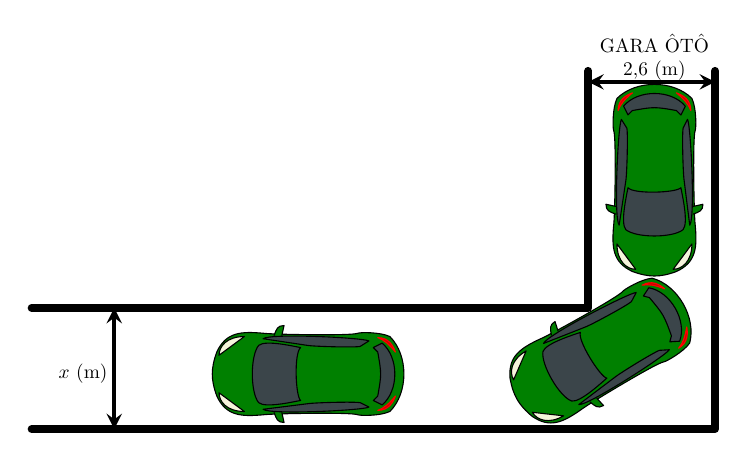
\begin{tikzpicture}[line join=round, line cap=round,scale=.7,transform shape,>=stealth]

			\tikzset{car/.pic={
						\def\T{
							(-2,1.85)
							..controls +(-10:.3) and +(-155:.3) ..(2.3,1.85)
							..controls +(25:.1) and +(155:.5) ..(3.75,1.7)
							..controls +(-45:1.2) and +(45:1.2) ..(3.75,-1.7)
							..controls +(-155:.5) and +(-25:.1) ..(2.3,-1.85)
							..controls +(155:.3) and +(10:.3) ..(-2,-1.85)
							..controls +(-175:1) and +(-65:1) ..(-4.1,-1)
							..controls +(110:.8) and +(-110:.8) ..(-4.1,1)
							..controls +(65:1) and +(175:1) ..(-2,1.85)
							;
						}
						\fill[ao(english)] \T;
						\draw[black]\T;

						\def\G{
							%Gương
							(-1.5,1.75)
							..controls +(70:.3) and +(180:.3) ..(-1.05,2.2)--(-1.15,1.75)

							(-1.5,-1.75)
							..controls +(-70:.3) and +(180:.3) ..(-1.05,-2.2)--(-1.15,-1.75)
							;}
						\fill[ao(english)] \G;
						\draw[black]\G;

						\def\K{
							(-2,1.6)
							..controls +(40:.4) and +(150:.3) ..(2.8,1.5) --(2.4,1.25)
							..controls +(-170:.3) and +(-10:.3) ..(0,1.3) --cycle

							(-2,-1.6)
							..controls +(-40:.4) and +(-150:.3) ..(2.8,-1.5)--(2.4,-1.3)
							..controls +(170:.3) and +(10:.3) ..(0,-1.35)--cycle

							(-2.2,1.3)
							..controls +(40:.4) and +(170:.3) ..(-.3,1.2)
							..controls +(-140:.4) and +(140:.3) ..(-.3,-1.2)
							..controls +(-170:.3) and +(-40:.4) ..(-2.2,-1.3)
							..controls +(130:.6) and +(-130:.6) ..cycle

							(3,1.2)--(3.4,1.4) %kính sau 
							..controls +(-40:1) and +(40:1) ..(3.4,-1.4)--(3,-1.2)--(3.2,-1)
							..controls +(80:1) and +(-80:1) ..(3.2,1)--(3,1.2)
						}

						\fill[arsenic] \K;
						\draw[black]\K;

						\def\D{ %Đèn trước
							(-4,.85)
							..controls +(90:.4) and +(180:.8) ..(-2.85,1.7) --cycle
							(-4,-.85)
							..controls +(-90:.4) and +(180:.8) ..(-2.85,-1.7) --cycle
							;
						}
						\fill[beige] \D;
						\draw[black]\D;
						%---------------------------
						\def\Ds{ %Đèn sau
							(4,1)
							..controls +(110:.3) and +(0:.5) ..(3.2,1.65)
							..controls +(-20:.3) and +(130:.5) ..cycle

							(4,-1)
							..controls +(-110:.3) and +(0:.5) ..(3.2,-1.65)
							..controls +(20:.3) and +(-130:.5) ..cycle
							;
						}
						\fill[bostonuniversityred] \Ds;
						\draw[red]\Ds;
					}}
			\path (6.3,.5)pic[rotate=90,scale=.4]{car}
			(5.3,-2.6)pic[rotate=30,scale=.4]{car}
			(0,-3)pic[scale=.4]{car};

			\draw[line width=1mm] (5.1,2.5)--(5.1,-1.8)--(-5,-1.8)
			(-5,-4)--(7.4,-4)--(7.4,2.5);

			\draw[line width=.5mm,<->] (-3.5,-1.8)--(-3.5,-4);
			\draw[line width=.5mm,<->] (5.1,2.3)--(7.4,2.3);

			\node[left] at (-3.5,-3){$x$ (m)};
			\node at (6.3,3){GARA ÔTÔ };
			\node at (6.3,2.5){$2{,}6$ (m)};
		\end{tikzpicture}
	\end{center}
	Đoạn đường đầu tiên có chiều rộng bằng $x$\,m, đoạn đường thẳng vào cổng gara có chiều rộng $2{,}6$\,m. Biết kích thước xe ô tô là $5$\,m $\times 1{,}9$\,m. Để tính toán và thiết kế đường đi cho ô tô người ta coi ô tô như một khối hộp chữ nhật có kích thước chiều dài $5$\,m, chiều rộng $1{,}9$\,m. Hỏi chiều rộng nhỏ nhất của đoạn đường đầu tiên bằng bao nhiêu mét để ô tô có thể đi vào gara được (kết quả làm tròn đến hàng phần mười)?
	\loigiai{
	Chọn hệ trục $Oxy$ như hình vẽ dưới.
	\begin{center}
		\definecolor{arsenic}{rgb}{0.23, 0.27, 0.29}
		\definecolor{ao(english)}{rgb}{0.0, 0.5, 0.0}
		\definecolor{bostonuniversityred}{rgb}{0.8, 0.0, 0.0}
		\definecolor{beige}{rgb}{0.96, 0.96, 0.86}
		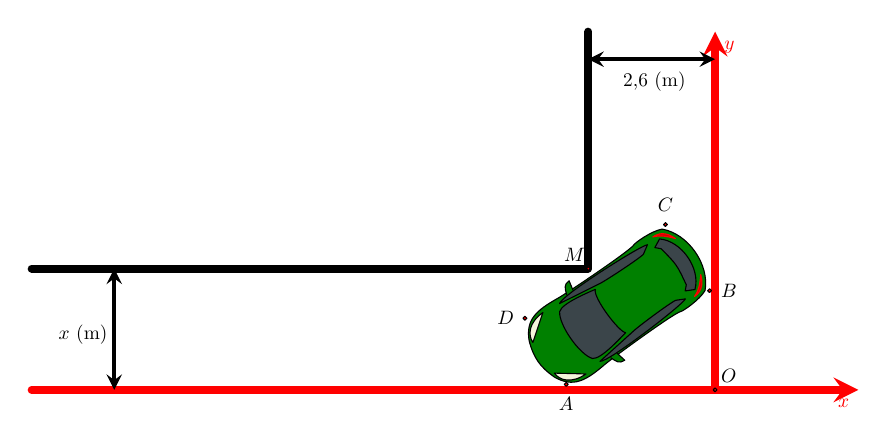
\begin{tikzpicture}[line join=round, line cap=round,scale=.7,transform shape,>=stealth]

			\tikzset{car/.pic={
						\def\T{
							(-2,1.85)
							..controls +(-10:.3) and +(-155:.3) ..(2.3,1.85)
							..controls +(25:.1) and +(155:.5) ..(3.75,1.7)
							..controls +(-45:1.2) and +(45:1.2) ..(3.75,-1.7)
							..controls +(-155:.5) and +(-25:.1) ..(2.3,-1.85)
							..controls +(155:.3) and +(10:.3) ..(-2,-1.85)
							..controls +(-175:1) and +(-65:1) ..(-4.1,-1)
							..controls +(110:.8) and +(-110:.8) ..(-4.1,1)
							..controls +(65:1) and +(175:1) ..(-2,1.85)
							;
						}
						\fill[ao(english)] \T;
						\draw[black]\T;

						\def\G{
							%Gương
							(-1.5,1.75)
							..controls +(70:.3) and +(180:.3) ..(-1.05,2.2)--(-1.15,1.75)

							(-1.5,-1.75)
							..controls +(-70:.3) and +(180:.3) ..(-1.05,-2.2)--(-1.15,-1.75)
							;}
						\fill[ao(english)] \G;
						\draw[black]\G;

						\def\K{
							(-2,1.6)
							..controls +(40:.4) and +(150:.3) ..(2.8,1.5) --(2.4,1.25)
							..controls +(-170:.3) and +(-10:.3) ..(0,1.3) --cycle

							(-2,-1.6)
							..controls +(-40:.4) and +(-150:.3) ..(2.8,-1.5)--(2.4,-1.3)
							..controls +(170:.3) and +(10:.3) ..(0,-1.35)--cycle

							(-2.2,1.3)
							..controls +(40:.4) and +(170:.3) ..(-.3,1.2)
							..controls +(-140:.4) and +(140:.3) ..(-.3,-1.2)
							..controls +(-170:.3) and +(-40:.4) ..(-2.2,-1.3)
							..controls +(130:.6) and +(-130:.6) ..cycle

							(3,1.2)--(3.4,1.4) %kính sau 
							..controls +(-40:1) and +(40:1) ..(3.4,-1.4)--(3,-1.2)--(3.2,-1)
							..controls +(80:1) and +(-80:1) ..(3.2,1)--(3,1.2)
						}

						\fill[arsenic] \K;
						\draw[black]\K;

						\def\D{ %Đèn trước
							(-4,.85)
							..controls +(90:.4) and +(180:.8) ..(-2.85,1.7) --cycle
							(-4,-.85)
							..controls +(-90:.4) and +(180:.8) ..(-2.85,-1.7) --cycle
							;
						}
						\fill[beige] \D;
						\draw[black]\D;
						%---------------------------
						\def\Ds{ %Đèn sau
							(4,1)
							..controls +(110:.3) and +(0:.5) ..(3.2,1.65)
							..controls +(-20:.3) and +(130:.5) ..cycle

							(4,-1)
							..controls +(-110:.3) and +(0:.5) ..(3.2,-1.65)
							..controls +(20:.3) and +(-130:.5) ..cycle
							;
						}
						\fill[bostonuniversityred] \Ds;
						\draw[red]\Ds;
					}}
			\path (5.6,-2.5)pic[rotate=35,scale=.4]{car}
			;

			\draw[line width=1mm] (5.1,2.5)--(5.1,-1.8)--(-5,-1.8)
			;
			\draw[red,->,line width=1mm] (-5,-4)--(10,-4)node[below left]{$x$};
			\draw[red,->,line width=1mm] (7.4,-4)--(7.4,2.5) node[below right]{$y$};

			\draw[line width=.5mm,<->] (-3.5,-1.8)--(-3.5,-4);
			\draw[line width=.5mm,<->] (5.1,2)--(7.4,2);

			\node[left] at (-3.5,-3){$x$ (m)};
			\node at (6.3,1.6){$2{,}6$ (m)};

			\path (7.4,-4)coordinate(O)
			(4.7,-3.9)coordinate(A)
			(7.3,-2.2)coordinate(B)
			(6.5,-1)coordinate(C)
			(3.95,-2.7)coordinate(D)
			(5.1,-1.8)coordinate(M)
			;
			\foreach \d/\g in {A/-90,B/0,C/90,D/180,O/45,M/135}{
					\draw[fill=red](\d) circle (1pt) +(\g:.35)node{$\d$};}

		\end{tikzpicture}
	\end{center}
	Khi đó $M(-2{,}6;x)$.\\
	Gọi $B(-a;0)$ suy ra $A\left(0 ; \sqrt{25-a^2}\right)$.\\
	Phương trình $A B\colon \dfrac{x}{-a}+\dfrac{y}{\sqrt{25-a^2}}-1=0$.\\
	Do $CD \parallel AB$ nên phương trình $CD\colon \dfrac{x}{-a}+\dfrac{y}{\sqrt{25-a^2}}-T=0$.\\
	Mà khoảng cách giữa $A B$ và $C D$ bằng $1{,}9$\,m nên
	\begin{align*}
		\dfrac{|T-1|}{\sqrt{\left(\dfrac{1}{a}\right)^2+\left(\dfrac{1}{\sqrt{25-a^2}}\right)^2}}=1{,}9 \Rightarrow T=1+\dfrac{9{,}5}{a \sqrt{25-a^2}}
	\end{align*}
	Điều kiện để ô tô đi qua được là $M$, $O$ nằm khác phía đối với bờ là đường thẳng $CD$.\\
	Suy ra $\dfrac{-2{,}6}{-a}+\dfrac{x}{\sqrt{25-a^2}}-1-\dfrac{9{,}5}{a \sqrt{25-a^2}} \geq 0 \Leftrightarrow x \geq \sqrt{25-a^2}+\dfrac{9{,}5}{a}-\dfrac{2{,}6 \times \sqrt{25-a^2}}{a}$.\\
	Ta có giá trị lớn nhất của hàm số $f(a)=\sqrt{25-a^2}+\dfrac{9{,}5}{a}-\dfrac{2{,}6 \times \sqrt{25-a^2}}{a}$ trên khoảng $(0;5)$ xấp xỉ $3{,}7$.\\
	Vậy chiều rộng nhỏ nhất của đoạn đường đầu tiên xấp xỉ $3{,}7$\,m.
	}
\end{bt}
% \label{De2}
% %
% \cleardoublepage
% \setcounter{page}{1}
% \rfoot{Trang \thepage/\pageref{DA2} - Đáp án trắc nghiệm Đề 2}
% \begin{center}
% 	\bfseries ĐÁP ÁN TRẮC NGHIỆM ĐỀ 2
% \end{center}

% \inputansbox{10}{ans/ansDe2-TN2}
% \label{DA2}
% %

